%this sections needs rewritten
%group it via question themed
%colour code tables - highlight significant results
%%%%%%%%%%%%%%%%%%%%%%%%%%%%%%%%%%%%%%%%%%%%%%%%%%%%%%%%%%%%%%%
\chapter{Results}

\section{Technological Systems Resilience}

Distinguishing technological and natural systems can be difficult in a landscape which has been actively shaped by its population for so long. The interaction between each of the systems of which the interplay results in the projected resilience is significant. For Trondheim the location of infrastructure including buildings and roads is the primary focus of the technological system which impact resilience to sea level extremes. How this infrastructure is built is of course of great importance to whether a speedy return to normality is possible after a sea level extreme event. Yet even perfectly designed infrastructure will still be impacted due to flooding. From the obvious  prevention of use during flooding, to post event clean up and the wear and damage which can occur from sea level extreme events.
\paragraph{}
The table below displays the number of building which are likely to be impacted during different sea level extremes in Trondheim. This is modelled by \cite{kartverket_se_2021} and was the base of later water level simulations as used in this project. Importantly this modelling is more localised than previous models of sea level extremes in Norway. 


\begin{table}[h]
    \centering
    \begin{tabular}{|l|l|l|l|l|}
    \hline
        water level & no. buildings  & ~ & ~ & ~ \\ \hline
        ~ & private & private & public  & critical  \\ \newline
        ~ & buildings & businesses & buildings & buildings \\ \hline        
        20 years return height now & 160 & 77 & 10 & 0 \\ \hline
        200 years return height now & 214 & 87 & 10 & 0 \\ \hline
        1000 years return height now & 242 & 104 & 14 & 0 \\ \hline
        Flooded 2090 & 66 & 51 & 8 & 0 \\ \hline
        20-years return height 2090 & 264 & 119 & 17 & 1 \\ \hline
        200-years return height  2090 & 308 & 136 & 24 & 1 \\ \hline
        1000-years return height  2090 & 332 & 148 & 26 & 1 \\ \hline
        1m sea level rise & 127 & 64 & 9 & 0 \\ \hline
        2m sea level rise & 343 & 155 & 29 & 1 \\ \hline
        3m sea level rise & 584 & 285 & 55 & 3 \\ \hline
        4m sea level rise & 752 & 335 & 70 & 5 \\ \hline
        5m sea level rise & 1023 & 402 & 77 & 8 \\ \hline
    \end{tabular}
    \caption{Impact of Sea Level Extremes - Buildings Flooded \cite{kartverket_se_2021} The major contrast between current 20 year storm surge and the 2090 20 year storm surge is that at this level a critical building is flooded. This would also occur at 2m sea level rise.}
    \label{building-impact-sle}
\end{table}
Table 4.1 shows that there is some risk from sea level extremes now. The 20 year return height is projected to cause the flooding of 247 buildings. However it is worth noting that no critical buildings are predicted to flood even with the 1000 year return height. This is in contrast to the 20 year return height in 2090, which is projected to cause the flooding of one critical building.

\paragraph{}
For many location the area of flooded land could be considered as falling within the natural systems, however Trondheim has a lot of reclaimed land, artificially straightened tidal rivers, protective harbours and managed coastlines. For this reason the amount of land which is projected to be flooded at different water levels is discussed within the technological systems resilience. Table 4.2 displays the non built up (natural areas) projected to be flooded along with the built upon lands.

\begin{table}[h]
    \centering
    \begin{tabular}{|l|l|l|l|l|l|l|}
    \hline
        water level & road & ~ & area  & ~ & ~ & ~ \\ \hline
                ~ & public & private & buildings & nature & primary & public \\ \newline
        ~ & road & road & ~ & ~ & industry &  facilities  \\ \hline
        20 years return height now & 980 & 1641 & 63684 & 657469 & 157153 & 3478 \\ \hline
        200 years return height now & 1296 & 1921 & 77215 & 734752 & 203260 & 4025 \\ \hline
        1000 years return height now & 1412 & 2391 & 86808 & 796016 & 235027 & 4633 \\ \hline
        Flooded 2090 & 893 & 182 & 35576 & 284492 & 27058 & 1799 \\ \hline
        20-years return height 2090 & 1532 & 3097 & 103637 & 895255 & 290125 & 6072 \\ \hline
        200-years return height  2090 & 2191 & 3634 & 163151 & 1012744 & 341126 & 10481 \\ \hline
        1000-years return height  2090 & 2596 & 3923 & 195742 & 1079657 & 374887 & 12312 \\ \hline
        1m sea level rise & 943 & 1118 & 51427 & 537291 & 99503 & 2815 \\ \hline
        2m sea level rise & 2676 & 3972 & 210415 & 1095157 & 376922 & 12617 \\ \hline
        3m sea level rise & 12896 & 6819 & 734367 & 1641854 & 768195 & 16690 \\ \hline
        4m sea level rise & 19136 & 8977 & 997157 & 2029422 & 1015730 & 32714 \\ \hline
        5m sea level rise & 24043 & 10539 & 1200656 & 2336924 & 1229702 & 37322 \\ \hline
    \end{tabular}
    \caption{Impact of Sea Level Extremes - Area Flooded  \cite{kartverket_se_2021}
    \label{area-impact-sle}
\end{table}

Road is measured in metres and Area is measured in metres squared. Considering Trondheim's coastal location this is not an particularly high amount of land projected to be impacted by various potential sea level extremes. However the location of so much key infrastructure within impact zones could be of concern in the coming future. 

Norway's economy is very dependent on activities along the coast\cite{aunan_strong_2008}, this is also the case for Trondheim. The information here will be used to discuss Trondheim's technological resilience to sea level extremes in the discussion. 


* For discussion - Conclusion of this : Trondheim is considered as having quite high technological system resilience to sea level extremes, but if it continues to place more and more infrastructure (particularly critical buildings) on the coast this will decrease. *

\section{Natural Systems Resilience}
map maps maps
geological map - resistance to erosion
DEM - height / steepness of coast line
how sea level change is occuring here
\paragraph{}
While Norway has large amounts of coastline, which could leave it vulnerable to sea level extremes \cite{aunan_strong_2008}, the natural coastline is not particularly vulnerable to inundation. The dominate Norwegian geological coastal setting includes resistant rock, steep slopes and high elevation, which provides a certain level of protection \cite{aunan_strong_2008}. 

Isostatic uplift also minimises the impact of rising sea levels in many locations, including Trondheimsfjord \cite{aunan_strong_2008}. Though the national level of natural protection is significant this is not the full story. Due to its wide variation and large levels of coastal infrastructure a more localised understanding of risk is required \cite{rod_integrated_2012}. 
\paragraph{}






From a natural system perspective of resilience Norway and Trondheim are likely to only have minimal impacts from increasing sea level extremes. However coastal cities may experience significant economic impacts \cite{aunan_strong_2008}

If repeating this research in a less urbanised environment land use should be considered. This was an excluded factor here due to \cite{hoffken_effects_2020} which showed that for highly urbanised environments characterising land use solely as land-surface vs water-surface was adequate when considering the impacts of storm surges.

\section{Social Systems Resilience}

%people underestimate current risk
%people overestimate future risk
%people care about climate - at least those who fill in survey

This chapter includes the summary statistics of the results gained from the survey conducted and the pilot survey. It also includes the results from Kruskal Wallis Tests and Shapiro Tests. Each of the results gained from the survey questions is displayed in a graph. These results will be discussed to determine Social Systems Resilience to Sea Level Extremes in the discussion. The tables and graphs below make reference to  the questions in the survey these results were gained from. For the full survey in either Norwegian or English please consult the appendix. Reference in text is only made to the English questions for ease of readability. 

\section{Pilot Survey and Focus Grop}

The pilot survey was conducted using 14 subjects who were classed as highly aware. They were asked seven questions and of them three of them included images of maps with questions which were used to attempt to determine subjects awareness. The figure below displays the results from the determination of awareness done on the pilot subjects.

\begin{figure}[h]
    \centering
    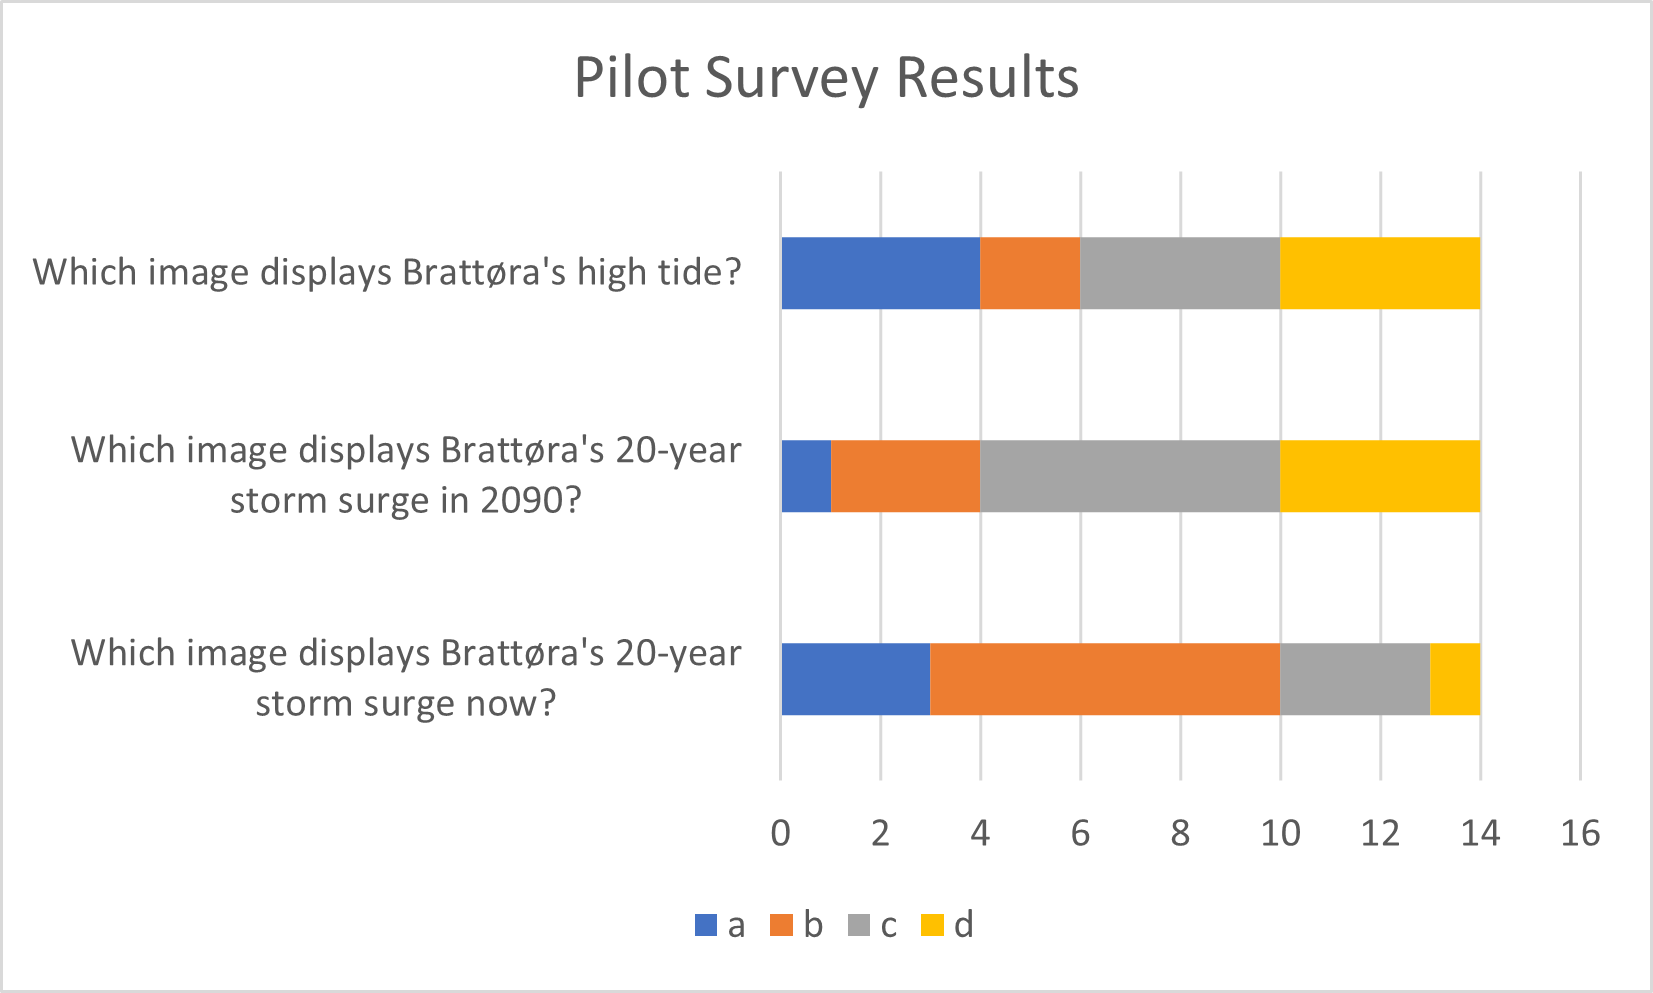
\includegraphics{fig_results/pilot-survey-results.png}
    \caption{Pilot Survey Results. The answers which matches the model \cite{kartverket_se_2021} were always B. This was done for ease of speedy analysis and discussion after survey completion. As can be seen the majority chose answer B for question "which image display's Brattøra's 20-year storm surge now". However for "Which image display's Brattøra's 20-year storm surge in 2090?" the majority chose C, with D the next popular answer   }
    \label{fig:pilot_survey_results}
\end{figure}

As can be seen in 

\section{Focus Group}





\section{Summary Statistics }
Find below table ** which details the summary statistics for the responses to the survey. Table ** contains the codified variable name and what questions they respond to .



\begin{center}
\begin{table}[h]
    \centering
    \begin{tabular}{|l|l|l|l|l|l|l|}
    \hline
        variable name & mean & Std Dev. & min & max & range & skew  \\ \hline
        long\_know & 3.24 & 1.60 & 0 & 6 & 6 & 0.23 \\ \hline
        com\_mem & 1.44 & 0.89 & 0 & 6 & 6 & 2.10  \\ \hline
        com\_marine\_worker & 0.00 & 0.00 & 0 & 0 & 0 & Na   \\ \hline
        com\_worker & 0.12 & 0.33 & 0 & 1 & 1 & 2.26  \\ \hline
        com\_resident & 0.46 & 0.50 & 0 & 1 & 1 & 0.17  \\ \hline
        com\_student & 0.25 & 0.44 & 0 & 1 & 1 & 1.11 \\ \hline
        com\_play\_land & 0.27 & 0.45 & 0 & 1 & 1 & 1.00   \\ \hline
        com\_play\_water & 0.11 & 0.32 & 0 & 1 & 1 & 2.45  \\ \hline
        com\_commuter & 0.10 & 0.31 & 0 & 1 & 1 & 2.56   \\ \hline
        com\_other & 0.12 & 0.32 & 0 & 1 & 1 & 2.35   \\ \hline
        interest\_level & 3.17 & 0.95 & 1 & 5 & 4 & -0.16 \\ \hline
        ss\_now & 0.39 & 0.49 & 0 & 1 & 1 & 0.44  \\ \hline
        ss\_future & 0.31 & 0.46 & 0 & 1 & 1 & 0.83 \\ \hline
        ss\_tide & 0.88 & 0.32 & 0 & 1 & 1 & -2.35 \\ \hline
        info\_place\_sum & 1.94 & 1.34 & 0 & 8 & 8 & 1.61 \\ \hline
        info\_climate\_sum & 3.50 & 1.72 & 0 & 8 & 8 & 0.24 \\ \hline
        worry\_climate & 4.03 & 1.15 & 1 & 5 & 4 & -1.17 \\ \hline
        flood\_impact & 2.50 & 0.89 & 1 & 4 & 3 & 0.04  \\ \hline
        slr\_past & 0.17 & 0.43 & 0 & 2 & 2 & 2.47  \\ \hline
        slr\_future & 2.33 & 0.69 & 0 & 3 & 3 & -1.26 \\ \hline
        ss\_event & 0.58 & 0.93 & 0 & 7 & 7 & 2.78  \\ \hline
        survey\_access & 2.55 & 1.84 & 0 & 6 & 6 & 0.79  \\ \hline
        language & 0.57 & 0.50 & 0 & 1 & 1 & -0.27  \\ \hline
        place\_brattøra & 0.20 & 0.40 & 0 & 1 & 1 & 1.52  \\ \hline
        place\_grillstad & 0.24 & 0.43 & 0 & 1 & 1 & 1.19 \\ \hline
        place\_nidelva & 0.37 & 0.49 & 0 & 1 & 1 & 0.52 \\ \hline
        place\_skansen & 0.19 & 0.39 & 0 & 1 & 1 & 1.57 \\ \hline
    \end{tabular}
    \caption{Summary Statistics}
\label{table:summary_stats}
\end{table}
\end{center}


\begin{center}
\begin{table}[h]
    \centering
    \begin{tabular}{|l|l|}
    \hline
        variable name  & question asked \\ \hline
        long\_know & How long have you known this area? \\ \hline
        com\_mem  & What communities in this area are you part of? \\ \hline
        com\_marine\_worker & "" \\ \hline
        com\_worker & "" \\ \hline
        com\_resident & "" \\ \hline
        com\_student & "" \\ \hline
        com\_play\_land & "" \\ \hline
        com\_play\_water &  "" \\ \hline
        com\_commuter &  "" \\ \hline
        com\_other &  "" \\ \hline
        interest\_level & What is your level of interest in sea level extremes? \\ \hline
        ss\_now  & Which image shows the current 20-year storm surge? \\ \hline
        ss\_future  & Which image shows the 20-year storm surge projected for 2090? \\ \hline
        ss\_tide  & Which image displays the current high tide? \\ \hline
        info\_place\_sum & Where do you get information about changes to this place? \\ \hline
        info\_climate\_sum &  "" \\ \hline
        worry\_climate &  Are you concerned about climate change? \\ \hline
        flood\_impact &  How would flooding associated with sea level extremes in this area affect you? \\ \hline
        slr\_past & How much do you think the sea level has changed here in the past 30 years? \\ \hline
        slr\_future & How much do you think the sea level will change in the next 30 years? \\ \hline
        ss\_event & Please tick if you remember any of these dates when coastal  \\ \newline
        & sea levels in Trondheim were over 2m \\ \hline
        survey\_access  & How did you access this survey? \\ \hline
        language  & Determined from which survey subjects filled out \\ \hline
        place\_brattøra  & "" \\ \hline
        place\_grillstad  & "" \\ \hline
        place\_nidelva & "" \\ \hline
        place\_skansen & "" \\ \hline
    \end{tabular}
    \caption{Variable link to Survey Question}
\label{table:variable to questions}
\end{table}
\end{center}


\begin{center}
\begin{table}[h]
    \centering
    \begin{tabular}{|l|l|l|l|l|l|l|}
    \hline
        variable name & mean & Std Dev. & min & max & range & skew  \\ \hline
        info\_place\_sum & 1.94 & 1.34 & 0 & 8 & 8 & 1.61 \\ \hline
        info\_place\_po & 0.73 & 0.45 & 0 & 1 & 1 & -1.00  \\ \hline
        info\_place\_family & 0.10 & 0.31 & 0 & 1 & 1 & 2.56 \\ \hline
        info\_place\_friend & 0.19 & 0.39 & 0 & 1 & 1 & 1.57  \\ \hline
        info\_place\_newspaper & 0.35 & 0.48 & 0 & 1 & 1 & 0.64  \\ \hline
        info\_place\_tv & 0.14 & 0.35 & 0 & 1 & 1 & 2.09 \\ \hline
        info\_place\_so\_me & 0.33 & 0.47 & 0 & 1 & 1 & 0.73  \\ \hline
        info\_place\_mem & 0.04 & 0.19 & 0 & 1 & 1 & 4.70 \\ \hline
        info\_place\_kommune & 0.07 & 0.26 & 0 & 1 & 1 & 3.28\\ \hline
        info\_climate\_sum & 3.50 & 1.72 & 0 & 8 & 8 & 0.24  \\ \hline
        info\_climate\_po & 0.45 & 0.50 & 0 & 1 & 1 & 0.20 \\ \hline
        info\_climate\_family & 0.18 & 0.38 & 0 & 1 & 1 & 1.68  \\ \hline
        info\_climate\_friend & 0.23 & 0.42 & 0 & 1 & 1 & 1.28  \\ \hline
        info\_climate\_newspaper & 0.72 & 0.45 & 0 & 1 & 1 & -0.96 \\ \hline
        info\_climate\_tv & 0.46 & 0.50 & 0 & 1 & 1 & 0.14 \\ \hline
        info\_climate\_so\_me & 0.63 & 0.48 & 0 & 1 & 1 & -0.55 \\ \hline
        info\_climate\_mem & 0.14 & 0.35 & 0 & 1 & 1 & 2.09 \\ \hline
        info\_climate\_sci & 0.39 & 0.49 & 0 & 1 & 1 & 0.44 \\ \hline
        info\_climate\_edu & 0.29 & 0.46 & 0 & 1 & 1 & 0.89 \\ \hline
        
         \end{tabular}
    \caption{Summary Statistics information access}
\label{table:summary_stats_info_access}
\end{table}
\end{center}

questions asked Where do you get information about this place? Where do you get information about climate change?
\begin{center}
\begin{table}[h]
    \centering
    \begin{tabular}{|l|l|l|l|l|l|l|}
    \hline
        variable name & mean & Std Dev. & min & max & range & skew \\ \hline
        risk\_p\_none & 0.46 & 2.10 & 0 & 10 & 10 & 4.31\\ \hline
        risk\_p\_he & 0.41 & 0.81 & 0 & 2 & 2 & 1.47 \\ \hline
        risk\_p\_drown & 0.72 & 0.96 & 0 & 2 & 2 & 0.58  \\ \hline
        risk\_p\_coldw & 0.24 & 0.65 & 0 & 2 & 2 & 2.35  \\ \hline
        risk\_p\_shore\_slide & 0.43 & 0.50 & 0 & 1 & 1 & 0.27 \\ \hline
        risk\_p\_ss & 0.57 & 0.50 & 0 & 1 & 1 & -0.27  \\ \hline
        risk\_p\_waves & 0.29 & 0.46 & 0 & 1 & 1 & 0.89 \\ \hline
        risk\_p\_wind & 0.34 & 0.48 & 0 & 1 & 1 & 0.67  \\ \hline
        risk\_p\_tide & 0.39 & 0.49 & 0 & 1 & 1 & 0.47  \\ \hline
        risk\_p\_storm\_total & 2.02 & 1.47 & 0 & 5 & 5 & 0.26  \\ \hline
        risk\_i\_dk & 0.72 & 2.59 & 0 & 10 & 10 & 3.28  \\ \hline
        risk\_i\_none & 0.26 & 1.60 & 0 & 10 & 10 & 5.88 \\ \hline
        risk\_i\_weathering & 1.08 & 1.44 & 0 & 3 & 3 & 0.58  \\ \hline
        risk\_i\_rain & 0.75 & 1.30 & 0 & 3 & 3 & 1.15\\ \hline
        risk\_i\_he & 0.35 & 0.76 & 0 & 2 & 2 & 1.68 \\ \hline
        risk\_i\_shore & 0.50 & 0.50 & 0 & 1 & 1 & -0.01 \\ \hline
        risk\_i\_ss & 0.63 & 0.48 & 0 & 1 & 1 & -0.55  \\ \hline
        risk\_i\_wave & 0.33 & 0.47 & 0 & 1 & 1 & 0.70  \\ \hline
        risk\_i\_wind & 0.31 & 0.46 & 0 & 1 & 1 & 0.83 \\ \hline
        risk\_i\_tide & 0.37 & 0.48 & 0 & 1 & 1 & 0.55  \\ \hline
        risk\_i\_storm\_total & 2.14 & 1.51 & 0 & 5 & 5 & 0.33 \\ \hline
          \end{tabular}
    \caption{Summary Statistics Perceived Risks}
\label{table:summary_stats_percieved_risks}
\end{table}
\end{center}

questions asked From the following what are the major risks to infrastructure in this area?
From the following what are the major risks to people in this area?

As can be seen in table* above the data is not normally distributed. This was confirmed by creating histograms for each value, searching for a normally distributed value which was independent to be the basis for analysis. 

\section{Awareness}

\section{factors}

\section{Community Membership}

t more non resident (83 subjects)
than residents (70 subjects) 

but perhaps people only ticked one box
next time more obvious tick all that apply

how did i access these non residents - can check

also could discuss views of those who consider themself inplace
as those who would tick resident 

i recon that could have got quite a few who were not resident in place - e.g. brattora doesnt have people who live there

but what do people think when they see resident 
- who ticks it
- are those people who i can consider as "inplace" with a greater impact on the creation of place

result from kruskal wallis test is that residence impacts awareness
but i have not shown how
like could be less aware
or more aware 

\section{Access to Survey}
words words
\begin{figure}[h]
    \centering
    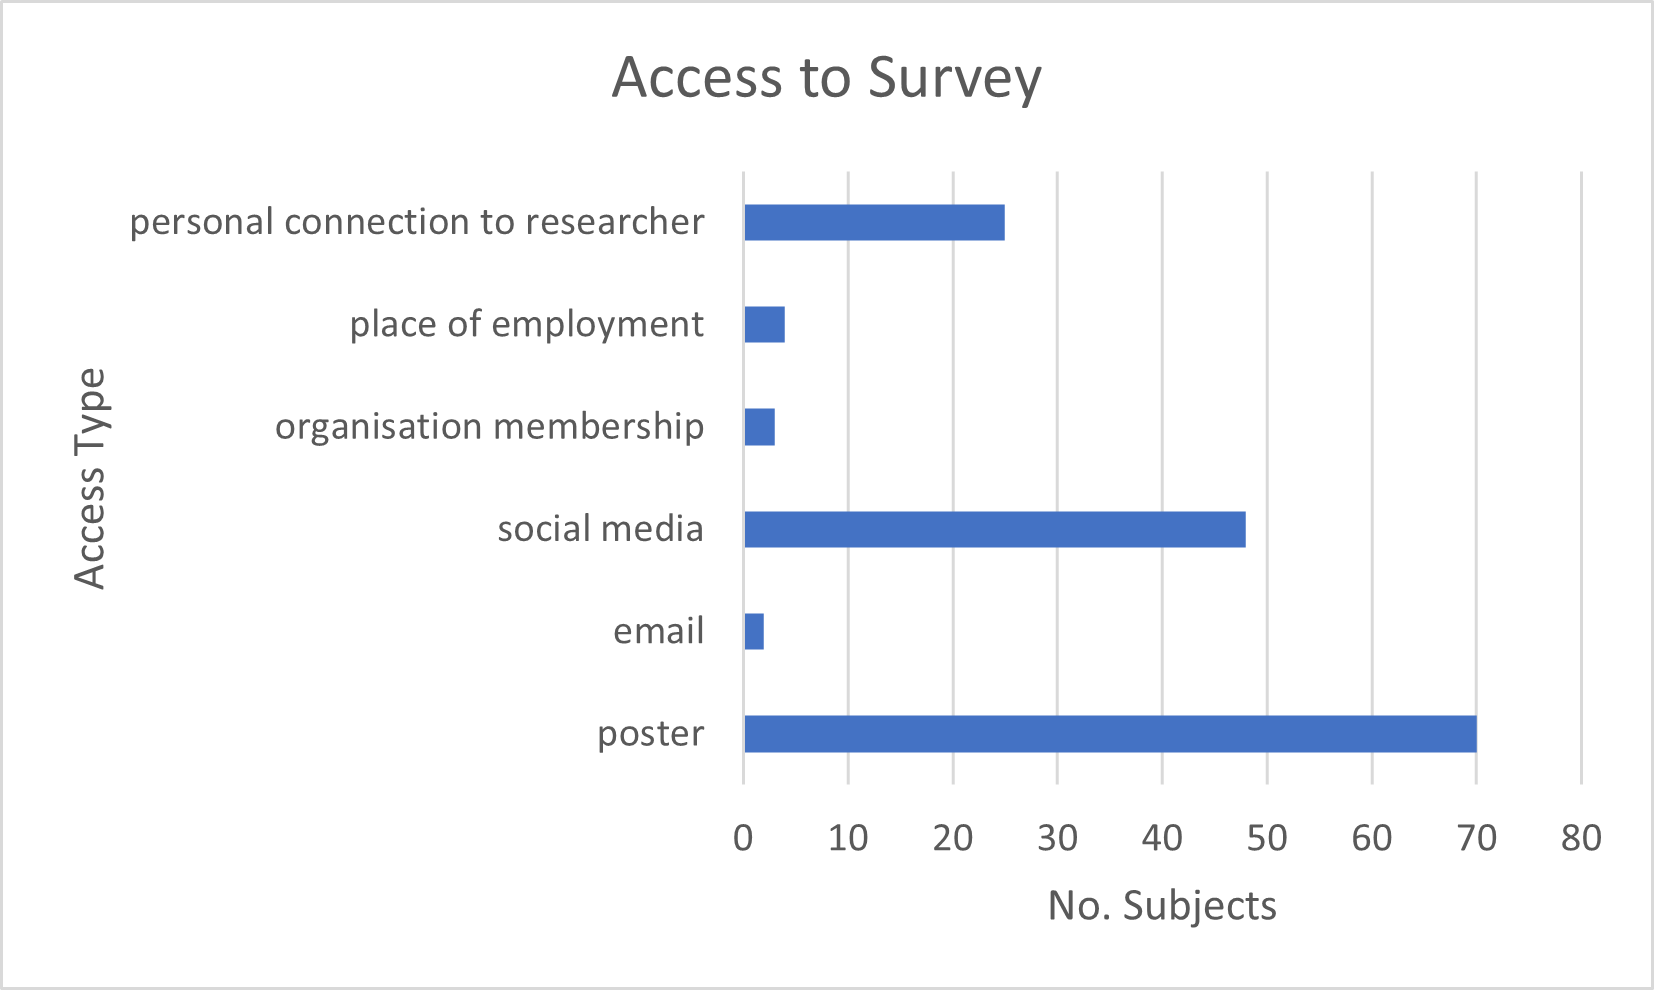
\includegraphics{fig_results/access_survey.png}
    \caption{Access to Survey. The most common access method of the survey was poster, with 70 subjects selecting this choice. This is followed by social media which has 47 subjects choosing this. Only 25 subjects accessed the survey due to personal connection to researcher. Access via email, place of employment and organisation membership are all under 10. Subjects could chose more than one access type. For example a subject could have accessed via personal connection to researcher and social media, due to the researcher sharing this survey on her personal page.}
    \label{fig:access_survey}
\end{figure}

\section{Experience of Sea Level Extremes}
that interest level doesnt factor with determined awareness is interesting, need it here so i can discuss in discussion 

\section{Histograms}
Awareness of changing sea levels is considered as the most important factor of local knowledge for resilience to sea level extremes. Five questions were asked which could make up the variable of awareness. These variables are ss-now, ss-future, ss-tide, slr-past, slr-future and the questions they are based off are outlined in table 5.2 - Variable link to Survey Question. As can be seen in table 5.1 - Summary Statistics these variables are individually very skewed. The original plan had been to combine all these answers to determine awareness. This variable is referred to as ss-aware-all and is in the 3rd graph in figure 5.1 Histogram Potential Awareness Variables. The other graphs show other attempts at creating a normally distributed variable which could be used in basic linear modelling to determine which factors influence awareness.

\begin{figure}[h]
    \centering
    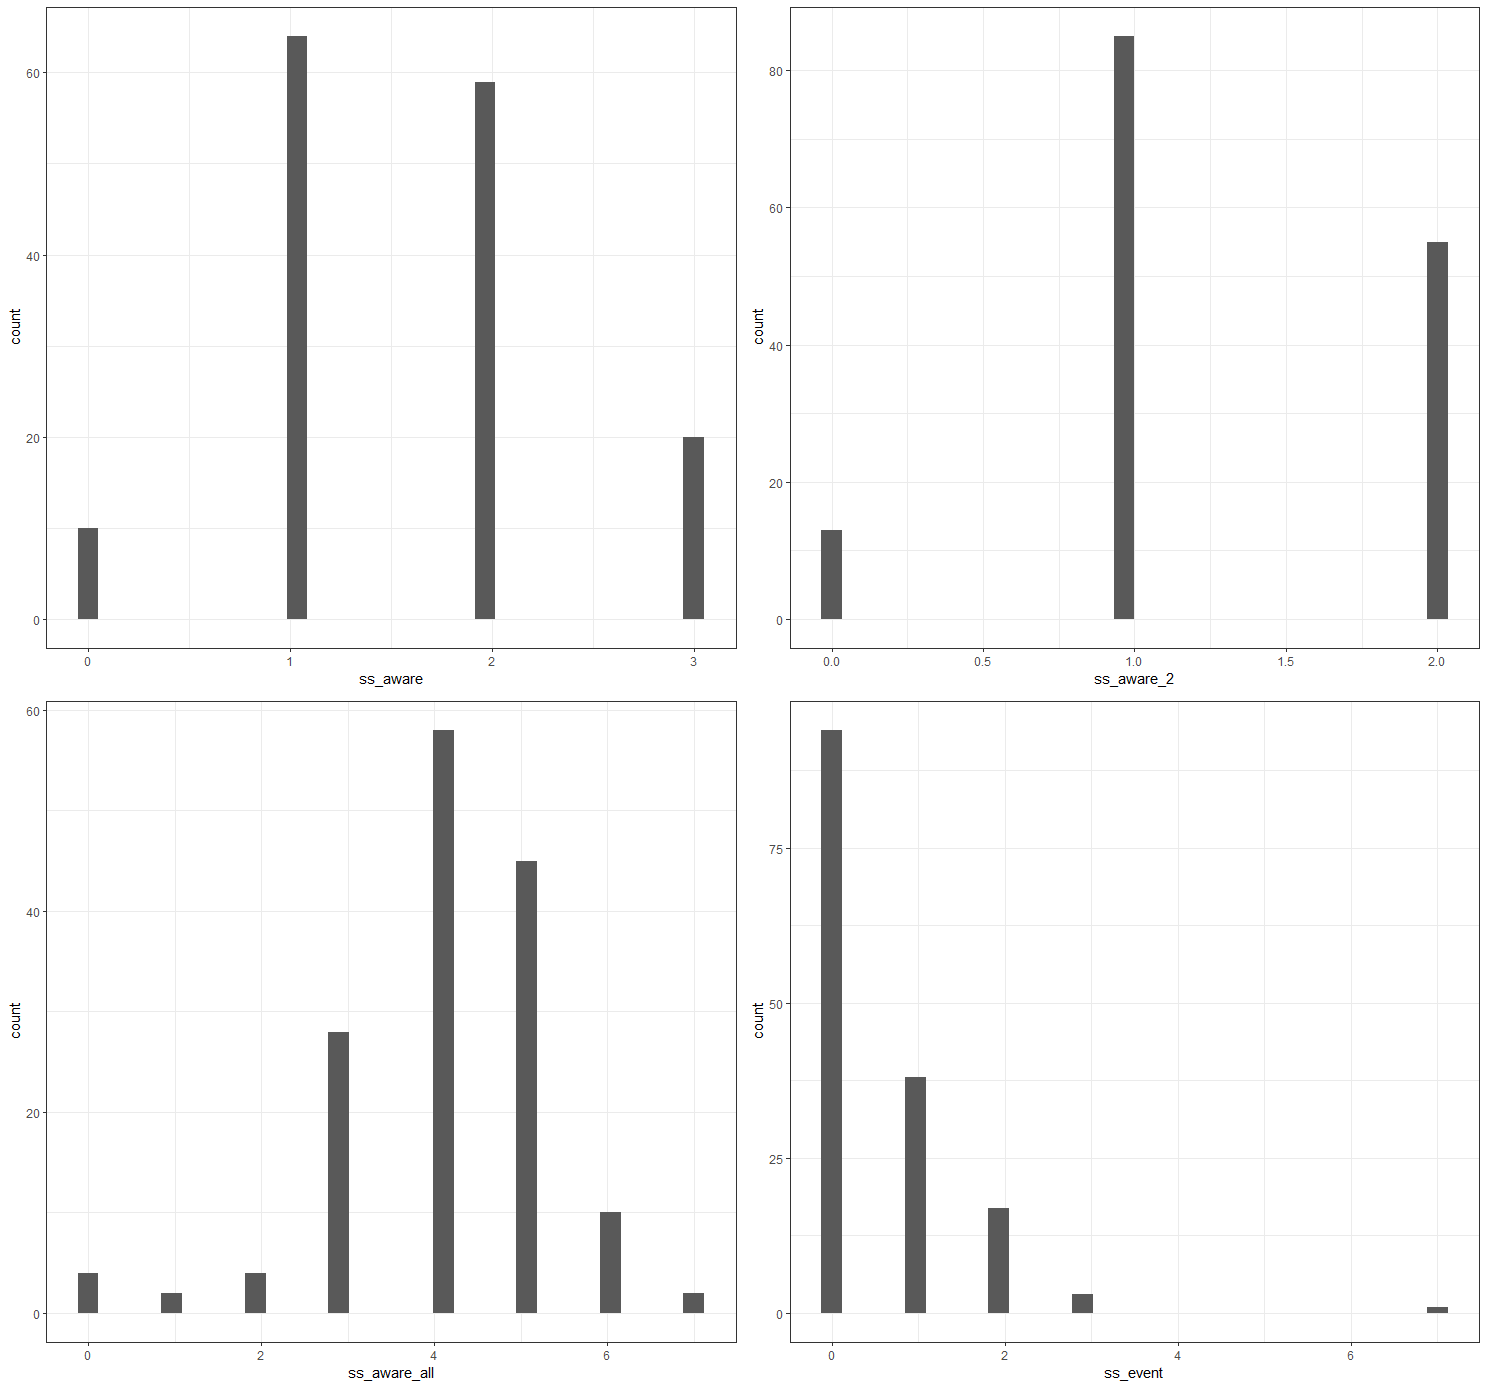
\includegraphics[width=1\textwidth]{fig_results/Awareness.png}
    \caption{Histogram Potential Awareness Variables}
    \label{fig:aware}
\end{figure}

Graph top left in the figure above displays the histogram for ss-aware variable which combined ss-now, ss-future and ss-tide. This was chosen as the most appropriate variable due to the fact that only awareness questions with a simulated water level picture were included, as can be seen in the appendix. While ss-aware-all is very skewed and the inclusion of two questions which are based purely off numeric answers is likely the reason for this. When given just numeric responses the accurate rate was non significant. For example only 3 subjects out of 153 gave the correct answer for slr-past, which is very unlikely given that it was multiple choice with only 7 potential answers (if split evenly then would have 21 subjects choosing this response. While slr-future had more correct responses, this was only mildly significant which combined the lack of correct answers for slr-past was seen as a good reason to exclude the answers to both of these questions for creating the variable of awareness. 

Graph top right displays the histogram for ss-aware-2 which only includes ss-now and ss-tide, excluding ss-future. This was considered as a potential baseline variable for current awareness to sea level extremes, however the variable summary statistics were incredibly simlar to ss-aware.

Graph bottom right displays the histogram for ss-event. This was expected to be a very skewed variable. Value 0 is the most common and displays the number of subjects with no memory of sea level extremes in Trondheim. Each other number indicates the number of sea level extreme events (water level higher than 2m) the subject remembered occurring between 1950 and summer 2022. For the full list of potential events please consults the relevant question in the appendix. This is included in this graph to show for how few subjects memory of a sea level extreme impacted their awareness. The lack of memory is very interesting considering that length of knowledge for the majority included two sea level extreme events. The histogram for long-know is the second graph in figure 5.2 Histogram Potential Factors below.

THIS ALSO ANSWERS RESEARCH Q 2
SUBJECTS ARE SOMEWHAT AWARE BUT NOT VERY


\begin{figure}[h]
    \centering
    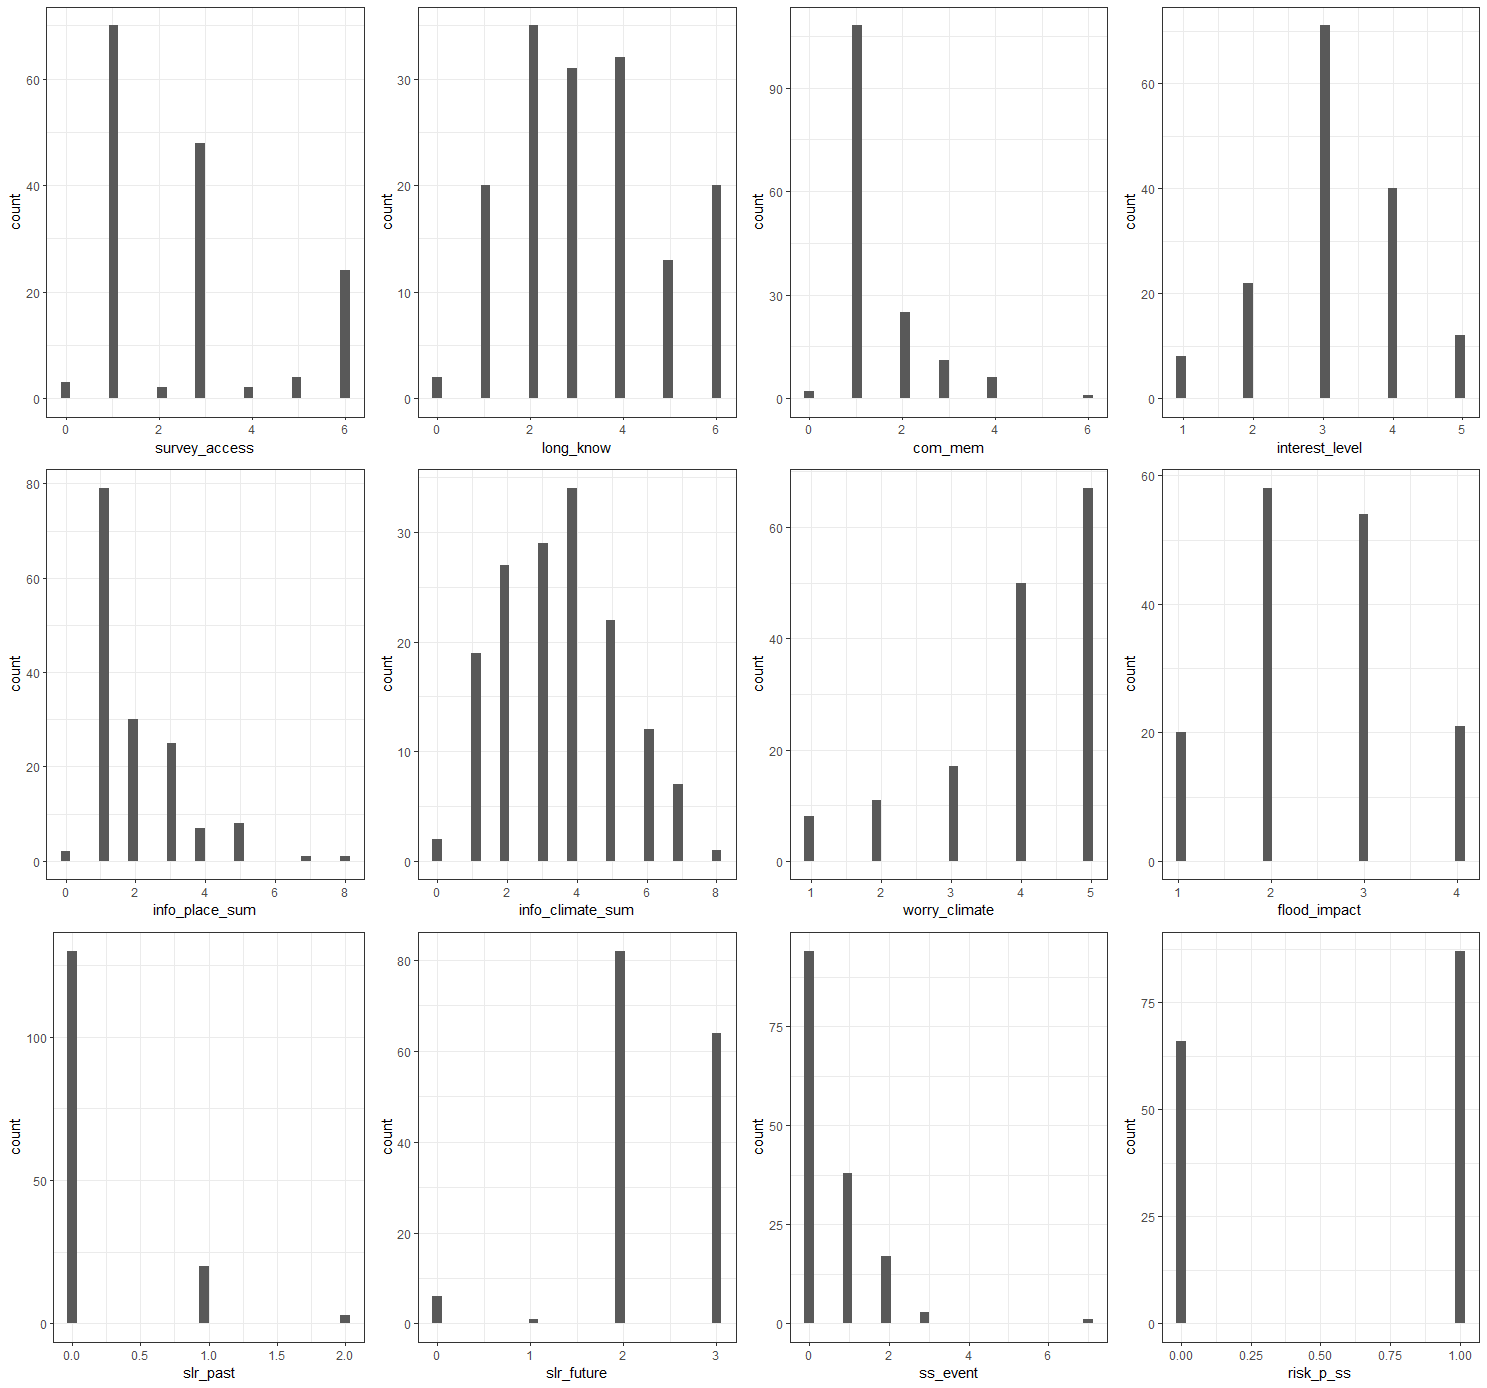
\includegraphics[width=1\textwidth]{fig_results/large_factors_all_histogram.png}
    \caption{Histogram Potential Factors}
    \label{fig:factors}
\end{figure}

As can be seen from this graph as well as all the awareness variable potentials being skewed so are the majority of the potential factors. The least skewed were long-know, interest-level and info-climate-sum. These factors then were tested using Shapiro test to determine whether they were as normally distributed as they seemed. 


\section{Shapiro Test Results}

During histogram analysis both the variables of "interest-level" and "info-sum-climate" appeared normally distributed. To investigate whether these variables were normally distributed or just appeared roughly to be a Shapiro test was carried out using**(royston 1982) . Due to inexperience with this method it was first checked on variables which from the histograms were clearly not normalised. From these tests and **(royston 1982) an assumption of alpha value of 0.05 was determined meaningful. This means if the p-value created during this test is below 0.05 then the null hypothesis is rejected. This does leave a 5 percent chance of error. The results from the Shapiro test can be seen in table* below and this determines that none of the variables were normally distributed. 

\begin{table}[h]
    \centering
    \begin{tabular}{|l|l|l|l|}
    \hline
         Variable & W-value & P-Value & Distribution \\ \hline
       Interest Level & 0.89332 & 4.343e-09 & Skewed \\ \hline
         Info Climate Sum  & 0.95721 & 0.0001159 & Skewed \\ \hline
        Flood Impact & 0.87779 & 6.681e-10 & Skewed \\ \hline
     \end{tabular}
    \caption{Shapiro Test Results. The alpha value was assigned 0.05, meaning that if the p-value is below 0.05 then the null hypothesis that this factor is not normally distributed was rejected. This leaves a 5 percent chance of error. Each of these factors p-value is below 0.05 meaning that their distribution was deemed skewed.}
    \label{table:shapiro_test_results}
\end{table}



\section{Kruskal Wallis Test Results}
Kruskal Wallis Rank Sum Test was conducted using R, specifically the package based off \cite{hollander_nonparametric_2014}. Kruskal Wallis Rank Sum Test was chosen due to the the distribution of the results and the potential interdependency of the data. Linear modelling was also considered and trialled, but this technique includes the skewed aspect of the data better, when looking for dependents. 
\begin{table}[h]
    \centering
    \begin{tabular}{|l|l|l|l|}
    \hline
         ~ & ss\_aware as predictor & ~ & ~ \\ \hline
        variable name & p value & h value & df \\ \hline
           long\_know & 0.73760 & 3.54770 & 6 \\ \hline
        com\_mem & 0.52060 & 4.20260 & 1 \\ \hline
        com\_marine\_worker & na & na & na \\ \hline
        com\_worker & 0.12310 & 2.37220 & 1 \\ \hline
        com\_resident & \cellcolor[HTML]{7df9ff} 0.01524 & 5.88900 & 1 \\ \hline
        com\_student & 0.55590 & 0.34691 & 1 \\ \hline
        com\_play\_land & 0.68790 & 0.16141 & 1 \\ \hline
        com\_play\_water & 0.42120 & 0.64690 & 1 \\ \hline
        com\_commuter & 0.44610 & 0.58063 & 1 \\ \hline
        com\_other & 0.58620 & 0.29627 & 1 \\ \hline
        interest\_level & 0.16920 & 6.43150 & 4 \\ \hline
        worry\_climate & 0.05630 & 9.19960 & 4 \\ \hline
    \end{tabular}
    \caption{Kruskal Wallis Test Results General Variables}
    \label{Kruskal_wallis_test_general}
\end{table}
com resident p value is below 0.05 hence dependent
worry climate p value is 0.05, so not necessarily relevant but very close, but h-value is particularly large hence may be dependent anyway

alpha of 0.05 indicates a 5 percent
risk of concluding that a difference exists when there is no actual difference.

As the P-value for the variable community membership -residence is greater than the alpha (could assign 0.05 as is common or assign 0.1 which would make it easier to include a few more variables for discussion) The differences between some of the medians are statistically significant.

\begin{table}[h]
    \centering
    \begin{tabular}{|l|l|l|l|l|l|l|}
    \hline
        variable name & p value & h value & df & p value & h value & df \\ \hline
        predictor & ss\_aware & ~ & ~ & ss\_aware\_2 & ~ & ~ \\ \hline
        info\_place\_sum & 0.44600 & 6.85110 & 7 & 0.45040 & 6.79650 & 7 \\ \hline
        info\_place\_po & 0.22730 & 1.45790 & 1 & 0.36470 & 0.82162 & 1 \\ \hline
        info\_place\_family & 0.78550 & 0.07406 & 1 & 0.81340 & 0.05572 & 1 \\ \hline
        info\_place\_friend & 0.27580 & 1.18780 & 1 & 0.30200 & 1.06520 & 1 \\ \hline
        info\_place\_newspaper & 0.74490 & 0.10583 & 1 & 0.48500 & 0.48765 & 1 \\ \hline
        info\_place\_tv & 0.87330 & 0.02542 & 1 & 0.33420 & 0.93237 & 1 \\ \hline
        info\_place\_so\_me & 0.48540 & 0.48671 & 1 & 0.95090 & 0.00379 & 1 \\ \hline
        info\_place\_mem & 0.67530 & 0.17550 & 1 & 0.70980 & 0.13848 & 1 \\ \hline
        info\_place\_kommune & 0.82590 & 0.04839 & 1 & 0.12790 & 0.57600 & 1 \\ \hline
        info\_climate\_sum & 0.91220 & 3.32660 & 8 & 0.45218 & 8.12040 & 8 \\ \hline
        info\_climate\_po & 0.11750 & 2.45020 & 1 & 0.24550 & 1.34870 & 1 \\ \hline
        info\_climate\_family & \cellcolor[HTML]{7df9ff} 0.00481 & 0.94470 & 1 & 0.56970 & 0.32313 & 1 \\ \hline
        info\_climate\_friend & 0.82460 & 0.04910 & 1 & 0.63010 & 0.23186 & 1 \\ \hline
        info\_climate\_newspaper & 0.09036 & 2.86790 & 1 & \cellcolor[HTML]{7df9ff} 0.01218 & 6.24830 & 1 \\ \hline
        info\_climate\_tv & 0.61230 & 0.25689 & 1 & 0.75000 & 0.10154 & 1 \\ \hline
        info\_climate\_so\_me & 0.74950 & 0.10960 & 1 & 0.92830 & 0.00809 & 1 \\ \hline
        info\_climate\_mem & 0.30270 & 1.06220 & 1 & 0.27500 & 1.91500 & 1 \\ \hline
        info\_climate\_sci & 0.88040 & 0.02650 & 1 & 0.12390 & 2.36760 & 1 \\ \hline
        info\_climate\_edu & 0.64850 & 0.20779 & 1 & \cellcolor[HTML]{7df9ff} 0.02438 & 5.06770 & 1 \\ \hline
    \end{tabular}
    \caption{Kruskal Wallis Test Results Variables on Information Access}
    \label{Kruskal_wallis_test_information}
\end{table}

Kruskal wallis test indicate that com-mem-resident is a factor for ss-aware, it could be a random factor, which would mean a more appropriate method than basic linear modelling is linear mixed effect modelling. Linear mixed effect modelling should consider com-resident as a random factor for ss-aware and for ss-aware-2, then infor-climate-edu and info-climate-newspaper may be random factors.

Info-climate-sum and com-mem included factors which influence the chosen baseline variable, but do not in and of themselves appear dependent from the kruskal wallis test. However it does highlight that these factors may be important considerations and are worth trialling with linear mixed effect modeeling.



%https://www.youtube.com/watch?v=QCqF-2E86r0

\section{Summary of Results}
